\documentclass[13pt,letterpaper]{article}

% Compile with XeLaTeX or LuaLaTeX.
\usepackage{iftex}
\ifPDFTeX
  \errmessage{Please compile this document with XeLaTeX or LuaLaTeX}
\fi
\usepackage{fontspec}
\IfFontExistsTF{Times New Roman}
  {\setmainfont{Times New Roman}}
  {\setmainfont{TeX Gyre Termes}} % metrically similar fallback if Times New Roman is unavailable
\setmonofont{DejaVu Sans Mono}
\usepackage[letterpaper,margin=1in]{geometry}
\usepackage{graphicx}
\usepackage{setspace}
\usepackage{titlesec}
\usepackage{tocloft}
\usepackage{hyperref}
\usepackage{enumitem}
\usepackage{booktabs}
\usepackage{tabularx}
\usepackage{longtable}
\usepackage{float}
\usepackage{caption}
\usepackage{xurl}
\hypersetup{hidelinks}
\setstretch{1.15}
\setlength{\parindent}{0pt}
\setlength{\parskip}{0.35em}
\setcounter{secnumdepth}{3}
\setcounter{tocdepth}{3}
\titleformat{\section}{\normalfont\bfseries\fontsize{16}{19}\selectfont}{\thesection.}{0.6em}{}
\titleformat{\subsection}{\normalfont\bfseries\fontsize{14}{17}\selectfont}{\thesubsection}{0.6em}{}
\titleformat{\subsubsection}{\normalfont\bfseries\fontsize{13}{16}\selectfont}{\thesubsubsection}{0.6em}{}

% Fill these fields before submission.
\newcommand{\ProjectTitle}{Secure IoT Gateway Simulation for Resource Sensing (SIGS-RS)}
\newcommand{\TeamMemberOne}{\textless TEAM MEMBER NAME 1\textgreater}
\newcommand{\RegisterNumberOne}{\textless REGISTER NUMBER 1\textgreater}
\newcommand{\TeamMemberTwo}{\textless TEAM MEMBER NAME 2\textgreater}
\newcommand{\RegisterNumberTwo}{\textless REGISTER NUMBER 2\textgreater}
\newcommand{\SubmissionMonth}{October 2026}

\begin{document}

% ---------------- Cover page (based on supplied BCSE301L format) ----------------
\begin{titlepage}
\thispagestyle{empty}
\vspace*{0.15in}
\noindent\rule{\linewidth}{2pt}
\vspace{0.65in}

\begin{center}
{\bfseries\fontsize{24}{29}\selectfont \ProjectTitle\par}
\vspace{0.55in}
{\large by\par}
\vspace{0.30in}

\begin{tabularx}{0.95\linewidth}{@{}X X@{}}
\centering \TeamMemberOne & \centering \TeamMemberTwo \tabularnewline
\centering \RegisterNumberOne & \centering \RegisterNumberTwo
\end{tabularx}

\vspace{0.65in}
{\large A project report submitted\par}
\vspace{0.15in}
{\large for the course of\par}
\vspace{0.15in}
{\bfseries\large BCSE301L--SOFTWARE ENGINEERING\par}
\vspace{0.15in}
{\large in\par}
\vspace{0.15in}
{\bfseries\large B. Tech. COMPUTER SCIENCE AND ENGINEERING\par}
\vspace{0.55in}

\includegraphics[width=2.6in]{vit_logo.png}
\vfill
{\bfseries\large \SubmissionMonth\par}
\end{center}
\end{titlepage}

\pagenumbering{roman}
\tableofcontents
\clearpage

\section*{Abstract}
\addcontentsline{toc}{section}{Abstract}
% Write a one-page abstract: problem, approach, implemented features, evaluation, limitations.

\clearpage
\pagenumbering{arabic}

\section{Introduction}
% Background, motivation, objectives, scope, contributions, report organization.

\section{Literature Survey / Related Work}
% Discuss only sources actually consulted. Cite them; do not invent references.

\section{Existing Work / System}
% Describe the baseline/problem and limitations, supported by the SRS and project context.

\section{Proposed Work / System}
% Describe SIGS-RS and distinguish implemented behavior from planned or unverified behavior.

\section{Software Requirements Specification (SRS)}
% Summarize scope, users, functional/nonfunctional requirements, REQ-* identifiers,
% BR-1 through BR-4, assumptions, constraints, and TBD items.
% Preserve the authoritative SRS wording/meaning. Do not silently rewrite requirements.
% If required by the course, append the original docs/SRS.pdf as a separate appendix.

\section{System Design / Architecture}
% Insert a verified architecture diagram and describe components, interfaces and data flow.

\section{Technology Stack}
% List only technologies confirmed in source/configuration.

\section{Working Modules}
% List the implemented modules and their responsibilities.

\section{Module Descriptions with Diagrams}
% Describe each major module with an accurate diagram and explanation.

\section{Test Plan and Test Suite}
% Include test strategy, representative cases, actual observed test results, skips and limits.

\section{Screenshots}
% Add genuine screenshots from the running application/demo. Use placeholders until captured.
% Do not fabricate screenshots or present mockups as real execution evidence.

\section{Conclusion}
% Summarize implemented outcomes and evidence without unsupported compliance claims.

\section{Future Work}
% Separate known limitations from proposed future improvements.

\section{References}
% Use real sources actually consulted. Prefer BibTeX or a consistent numbered citation style.

\appendix
\section{Implementation}
% Add selected code listings, configuration excerpts, API examples, and run commands.
% Avoid dumping the entire repository into the report.

% Optional: append the authoritative SRS PDF verbatim if required by the instructor.
% Uncomment after placing the SRS PDF at the specified path and confirming course requirements:
% \usepackage{pdfpages} % move this package to the preamble
% 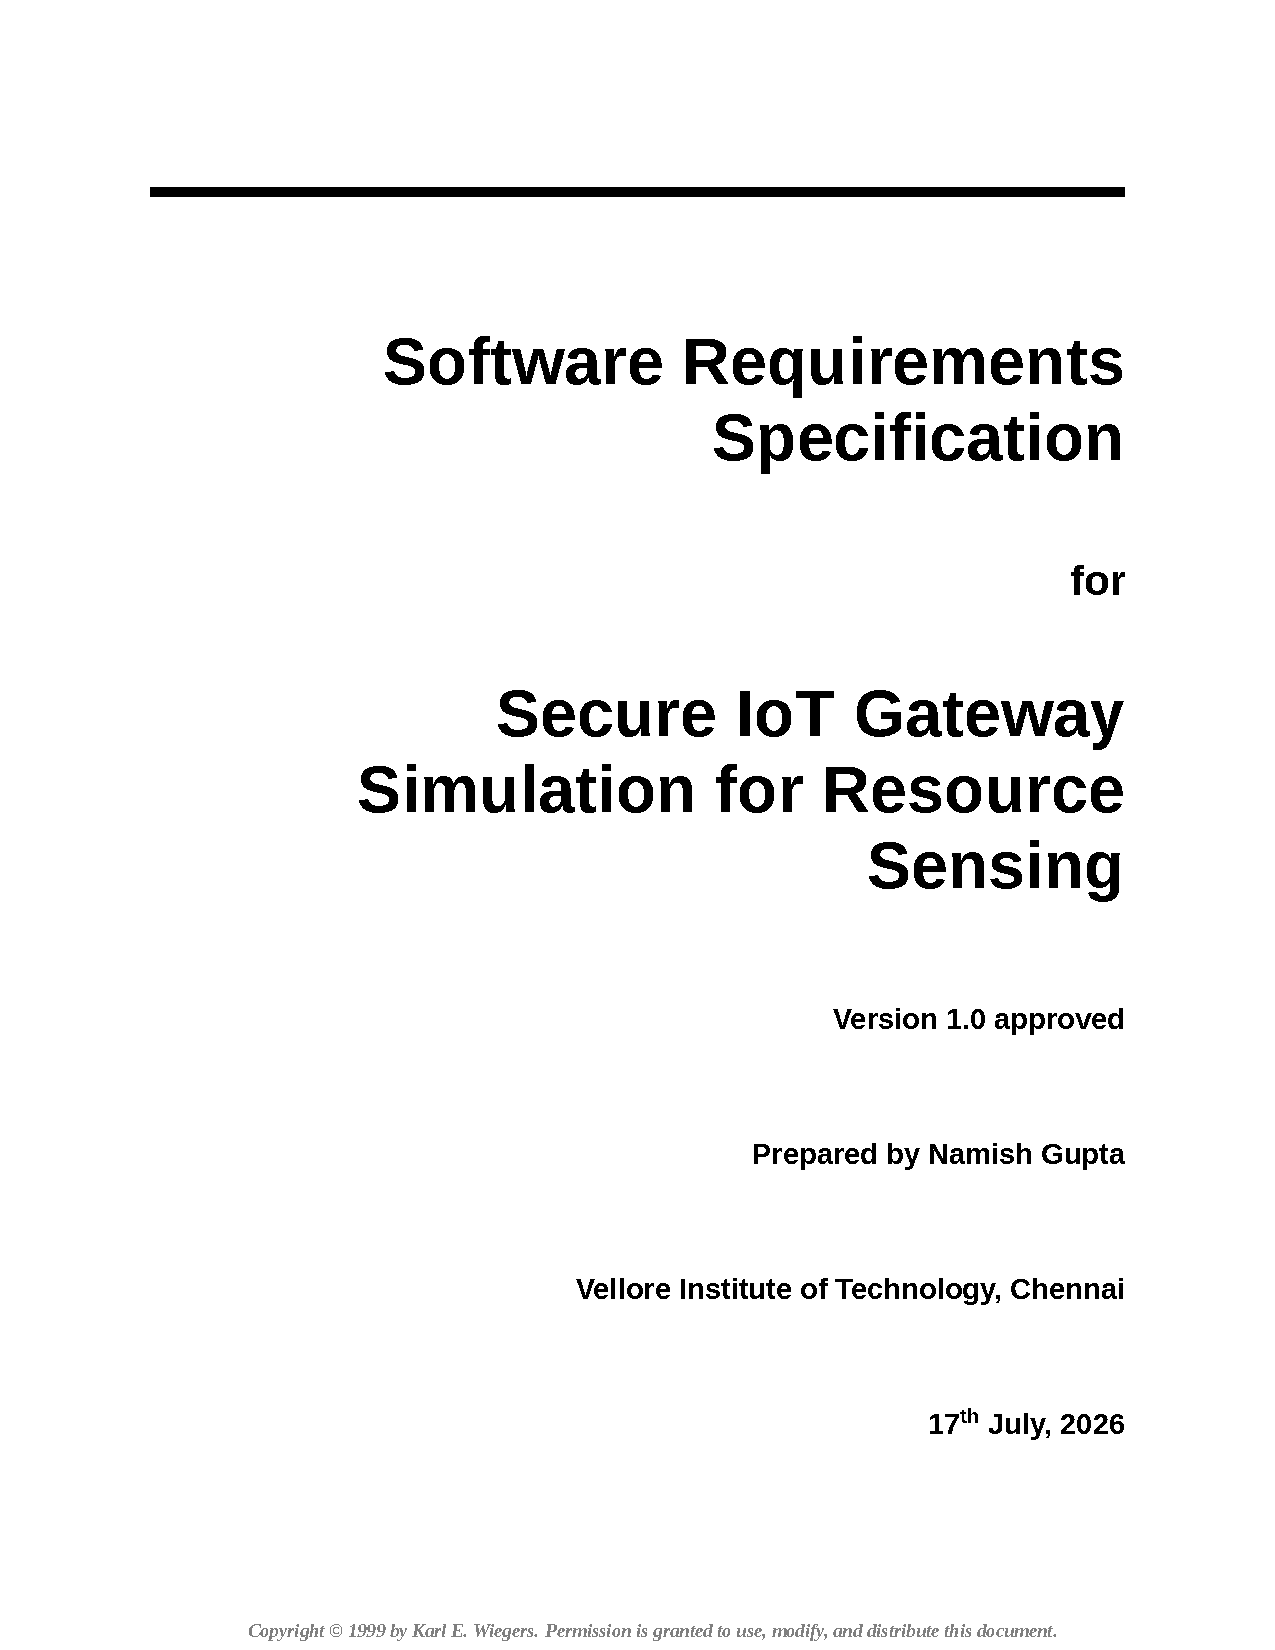
\includepdf[pages=-,pagecommand={\thispagestyle{plain}}]{../docs/SRS.pdf}

\end{document}
